\documentclass{article}
\usepackage[utf8]{inputenc}
\usepackage[czech]{babel}
\usepackage{multirow}
\usepackage{tikz}
\usepackage{lscape}
\usepackage{rotating}
\usepackage{graphicx}
\graphicspath{ {./images/} }

\usepackage[%
    left=1.50in,%
    right=1.50in,%
    top=1.0in,%
    bottom=1.0in,%
    paperheight=11in,%
    paperwidth=8.5in%
]{geometry}%

\setlength{\parskip}{\baselineskip}%
\setlength{\parindent}{0pt}%

\title{Dokument zadavatele \\ Sigma Male Flowers s.r.o.}
\author{Denis Akopyan, Jiří Otoupal, Sergei Naumenko, Oleg Veres, Jiří Vrba}
\date{4IT216 - ZS 2021/2022}

\begin{document}

\maketitle
\clearpage

\section*{Charakteristika firmy}

Firma Sigma Male Flowers s.r.o. (také jako $\Sigma$ Male Flowers) podniká v České republice od roku 2010.
Má momentálně 2 pobočky/prodejny, jednu v Praze a jednu v Brně.
Firma má dohromady přibližně 30 zaměstnanců, s tím, že stálých zaměstnanců je tam přibližně 20, zbytek
jsou brigádnící a pracovníci na DPP, DPČ.

Ve firmě pracuje několik typů pracovníků: floristé, zákaznická podpora, kurýři a oddělení logistiky.

Firma nakupuje květiny levně na burzách v Holandsku a následně si objednává jejich dopravu do České Republiky a zde je prodává s marží. Díky levné nákupní ceně mohou pořádat speciální akce a prodávat květiny levněji než většina konkurence.

Firma provozuje jak kamenné prodejny, kde si mohou zákazníci z ulice zakoupit květiny bez předchozího objednání, tak e-shop, kde je možné si objednat květiny a následně si je buď nechat dovézt nebo si je vyzvednout osobně.
Firma také spolupracuje s rozvážkovou službou DámeKytky.cz s.r.o. která pro ně zajišťuje objednávání a následný rozvoz květin po Praze.
Rozvoz je v rámci celé České Republiky do 24 hodin a za poplatek, v případě Brna a Prahy pak do 6 hodin od objednání a zdarma.

Aby bylo možné květiny uchovávat, provozují obě položky sklad se sníženou teplotou.
Je potřeba evidovat, jaké a kolik květin se v každém skladu nachází, aby bylo možné včas nakoupit docházející druh v požadovaném množství.
K tomu slouží sdílená Excel tabulka, do které zapisují zaměstnanci floristé odpisy při vyřizování objednávek a naopak zaměstnanci z oddělení logistiky zapisují přírůstky množství jednotlivých typů při převzetí objednávky.

Všechny objednávky (jak z e-shopu a DámeKytky.cz, tak od zákazníků v kamenné prodejně) se zapisují do hromadné sdílené Excel tabulky, aby pak bylo možné objednávky vyřizovat floristy a následně je zahrnout do účetnictví.

Na základě objednávek pak pracovníci z oddělení marketingu ručně hledají vzory chování, aby mohli zvyšovat efektivitu budoucích marketingových kampaní. Celkově má firma velký potenciál pro těžbu znalostí ze svých dat.

Floristé potřebují vědět, jaké objednávky mají vázat z jakého množství květin.
Objednávky se vyřizují prioritně podle času vyzvednutí / předání kurýrovi a podle velikosti objednávky.
Objednávky s větším počtem květů se vyřizují přednostně před objednávkami s malým počtem.

Zákaznická podpora zpracovává dotazy od uživatelů e-shopu, komunikuje s nimi v reálném čase pomocí chatu a přijímá objednávky po telefonu.

Kurýři rozvážejí objednávky a potřebují znát optimalizované trasy (v ideálním případě všechny objednávky v jedné lokalitě rozvážet najednou)

Pracovníci logistiky plánují trasy kurýrů, zajišťují zásoby zboží na skladě, v případě potřeby vytváří objednávky u obchodníků na Holandské burze a zajišťují dopravu do České Republiky.

\section*{Vize}

Firma má v plánu do budoucna expandovat pole svojí působnosti do dalších částí České Republiky
a otevřít nové pobočky v Ostravě, Plzni a Liberci. Dále má v plánu zvyšovat objem objednávek a tím
pádem i zvýšit svůj obrat a zisky z přidané marže.

K tomu, aby byla firma schopná expandovat potřebuje ale investovat do IT a potřebuje centrální systém, protože bez něj by bylo velice obtížné zvládat nárůst administrační a logistické zátěže.

Momentální stav IT ve firmě neumožňuje být dostatečně flexibilní a je jedním z hlavních faktorů bránící rozvoji.

Firma má také do budoucna plány zefektivnit svůj proces příjmání nových zaměnstnanců a management brigádníků v období nadměrného zatížení (např. Den matek nebo svátek sv. Valentýna, kdy vytíženost firmy přesahuje několikanásobně průměr)

\section*{Poslání}

Posláním společnosti je zpřístupnit široké veřejnosti květiny vysoké kvality, ale zároveň zachovat nízkou cenu.
Společnost se snaží cílit na velice obsáhlou cílovou skupinu, ale zároveň se snaží posílit svojí pozici na trhu s květinami pomocí speciálně cílených marketingových kampaní. V České Republice je vysoká konkurence a proto je potřeba pečlivě volit prodejní strategii a stanovování cen.

\clearpage


\section*{SWOT Analýza společnosti}

SWOT analýza je jednou z nejčastějších metod strategické analýzy.
Skládá se ze čtyř částí:
\begin{itemize}
    \item \textbf{S}trenghts - silné stránky společnosti
    \item \textbf{W}eaknesses - slabé stránky společnosti
    \item \textbf{O}pportunities - potencionální příležitosti
    \item \textbf{T}hreats - hrozby pro společnost
\end{itemize}

\begin{table*}[h]
    \begin{tabular}{|p{195pt}|p{195pt}|}
        \hline \bfseries Strengths &\bfseries Weaknesses  \\
        \hline
        {\begin{itemize}
            \item Kvalifikovaný personál floristů
            \item Kvalita produktu
            \item Individuální přístup k zákazníkům
            \item Stabilní supply chain + distribuce
        \end{itemize}}
        &
        {\begin{itemize}
            \item Nízké povědomí o firmě
            \item Prodej zboží s nízkou trvanlivostí
            \item Vysoké náklady na skladování
            \item Závislost na ekologických faktorech
            \item Informační šum mezi zaměstnanci
        \end{itemize}} \\
        \hline \bfseries Opportunities &\bfseries Threats  \\
        \hline
        {\begin{itemize}
            \item Květinové dekorace na oslavy a svatby
            \item Propojení s jinýmy službami poskytující rozvoz (Messenger, Bolt)
            \item Flower mystery boxes
        \end{itemize}} &
        {\begin{itemize}
            \item Vstup nové konkurence
            \item Upadající zájem ze strany zákazníků
            \item Legislativní změny (např. clo)
            \item Administrativní náročnost
        \end{itemize}} \\
        \hline
    \end{tabular}
\end{table*}

\section*{Byznys cíle společnosti}
\begin{itemize}
    \item Zvýšit podíl na českém trhu s květinami z 5\% na 16\% v průběhu maximálně 2 let
    \item Zvýšit efektivitu produkce a snížit čas potřebný na vyřízení objednávky o 10\%
    \item Zlepšit flexibilitu společnosti - snížit administrativní náklady a čas potřebný k náboru nových zaměstnanců o 30\%
    \item Zvýšit kapacitu objednávek o 20\% do konce roku 2022
    \item Rozšířit firmu o 1 pobočku do konce roku 2023 a o další 2 pak do 3 let
\end{itemize}

\clearpage

\section*{Business Model Canvas}
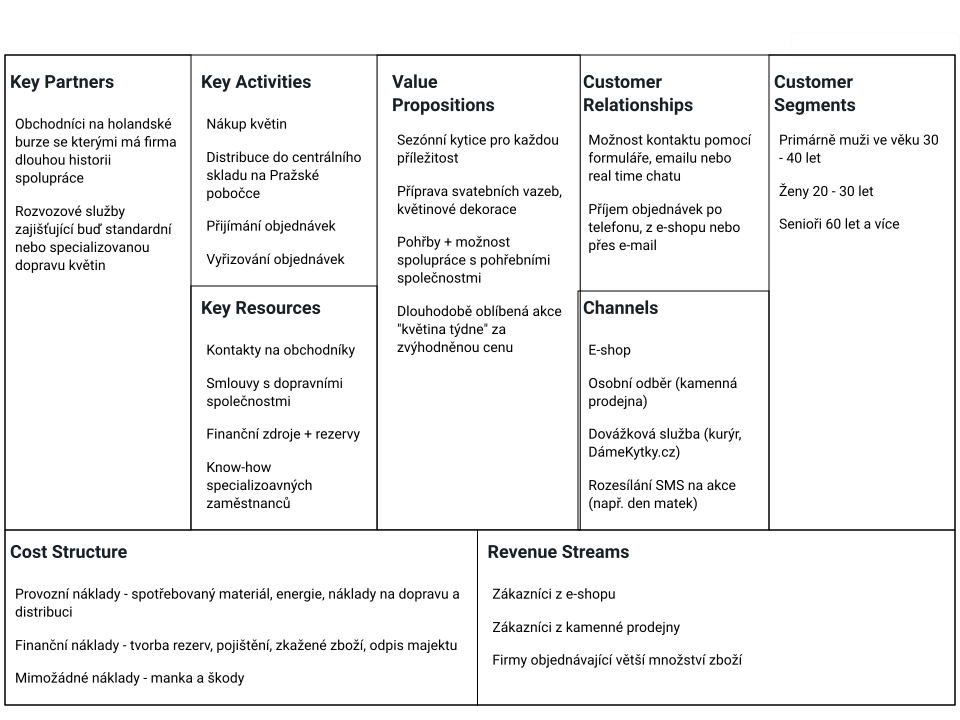
\includegraphics[width=\linewidth]{images/bmc.png}

\newpage

\section*{Popis současného stavu}

\subsection*{Procesy ve firmě}

\begin{figure}[h]
\caption{Objednávka květin na Holandské burze + vytvoření objednávky u dodavatele}
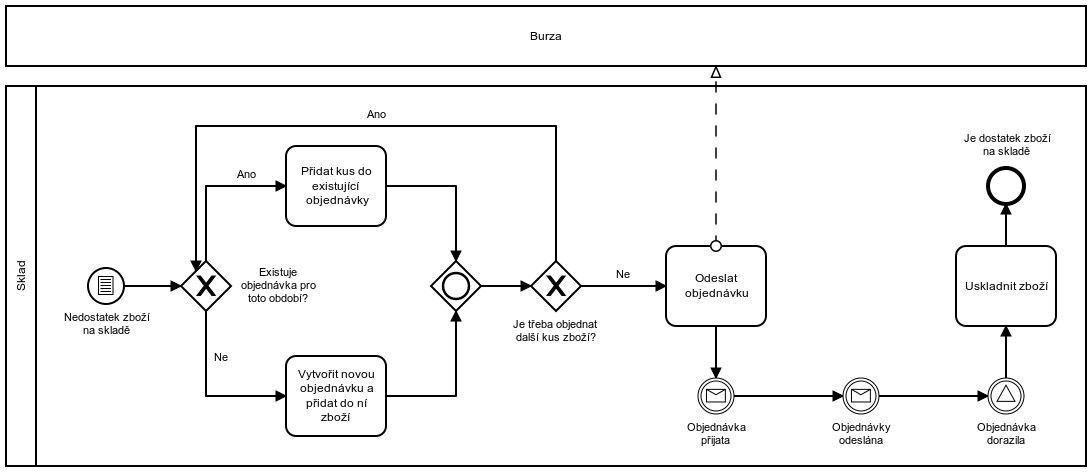
\includegraphics[width=\linewidth]{images/procesy/1.png}
\end{figure}

\newpage
\begin{figure}[h]
\caption{Doprava zboží z Holandska do České Republiky}
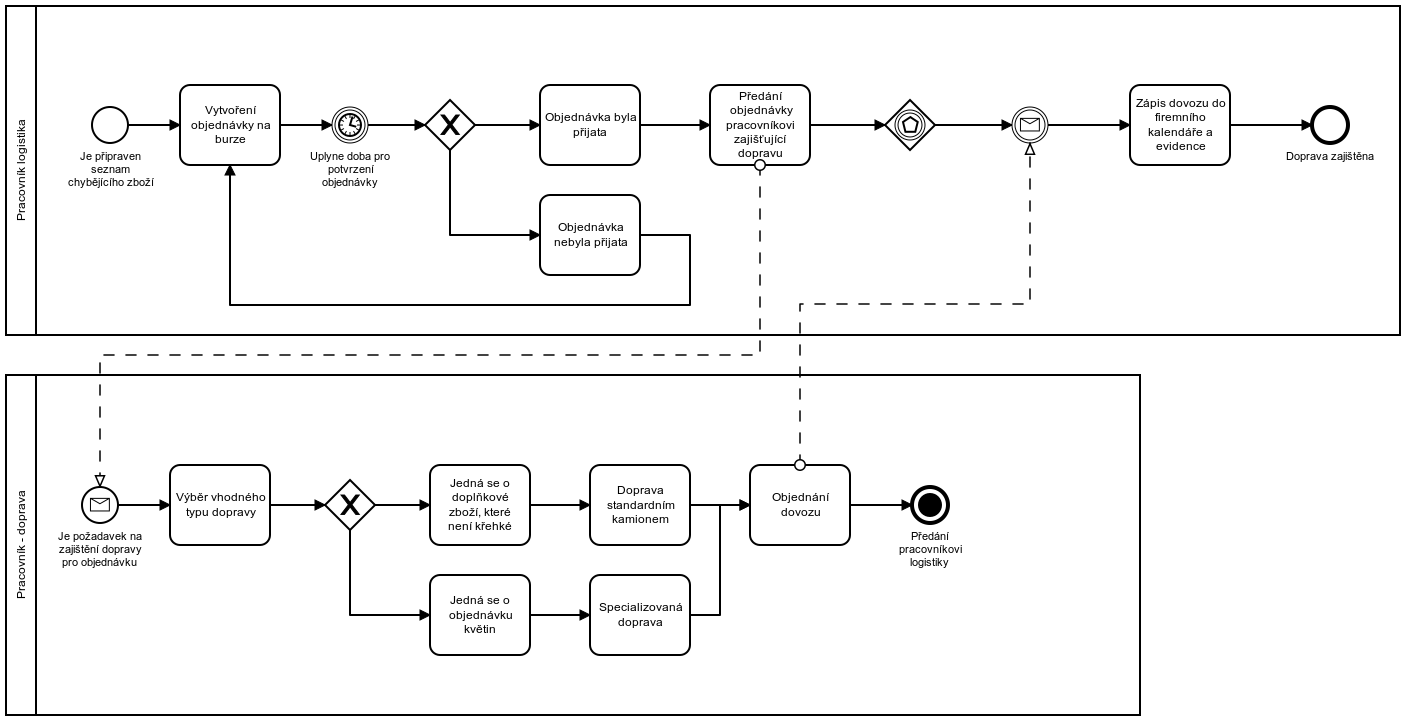
\includegraphics[width=\linewidth]{images/procesy/2.png}
\end{figure}

\newpage
\begin{figure}[h]
\caption{Distribuce zboží do ostatních poboček}
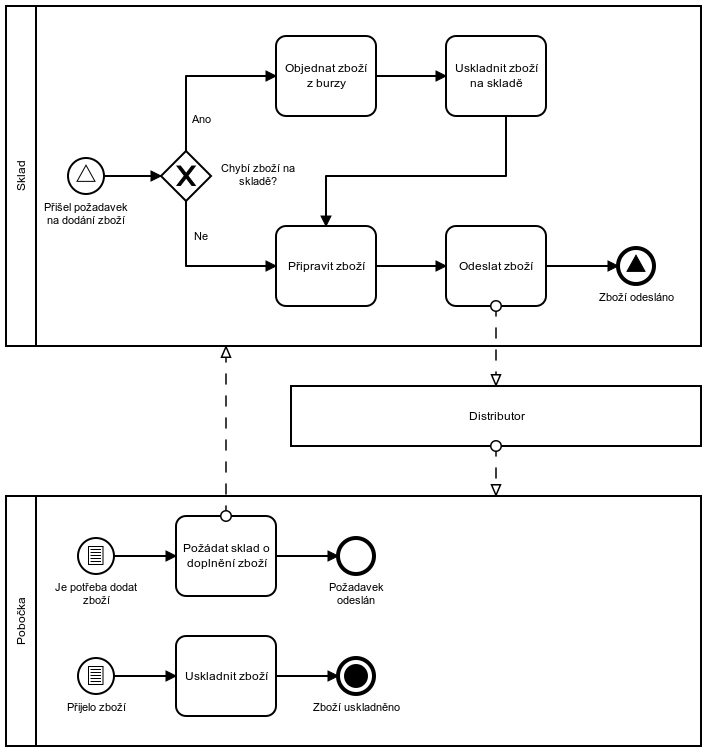
\includegraphics[width=\linewidth]{images/procesy/3.png}
\end{figure}

\newpage
\begin{figure}[h]
\caption{Vytvoření objednávky v kamenném obchodě}
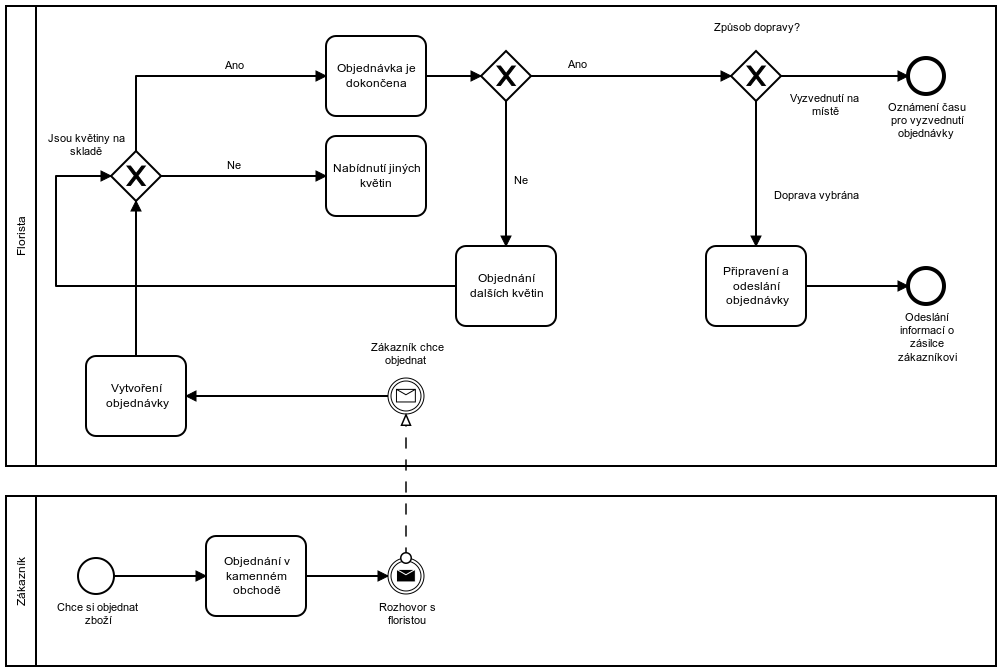
\includegraphics[width=\linewidth]{images/procesy/4.png}
\end{figure}

\newpage
\begin{figure}[h]
\caption{Vytvoření objednávky na e-shopu}
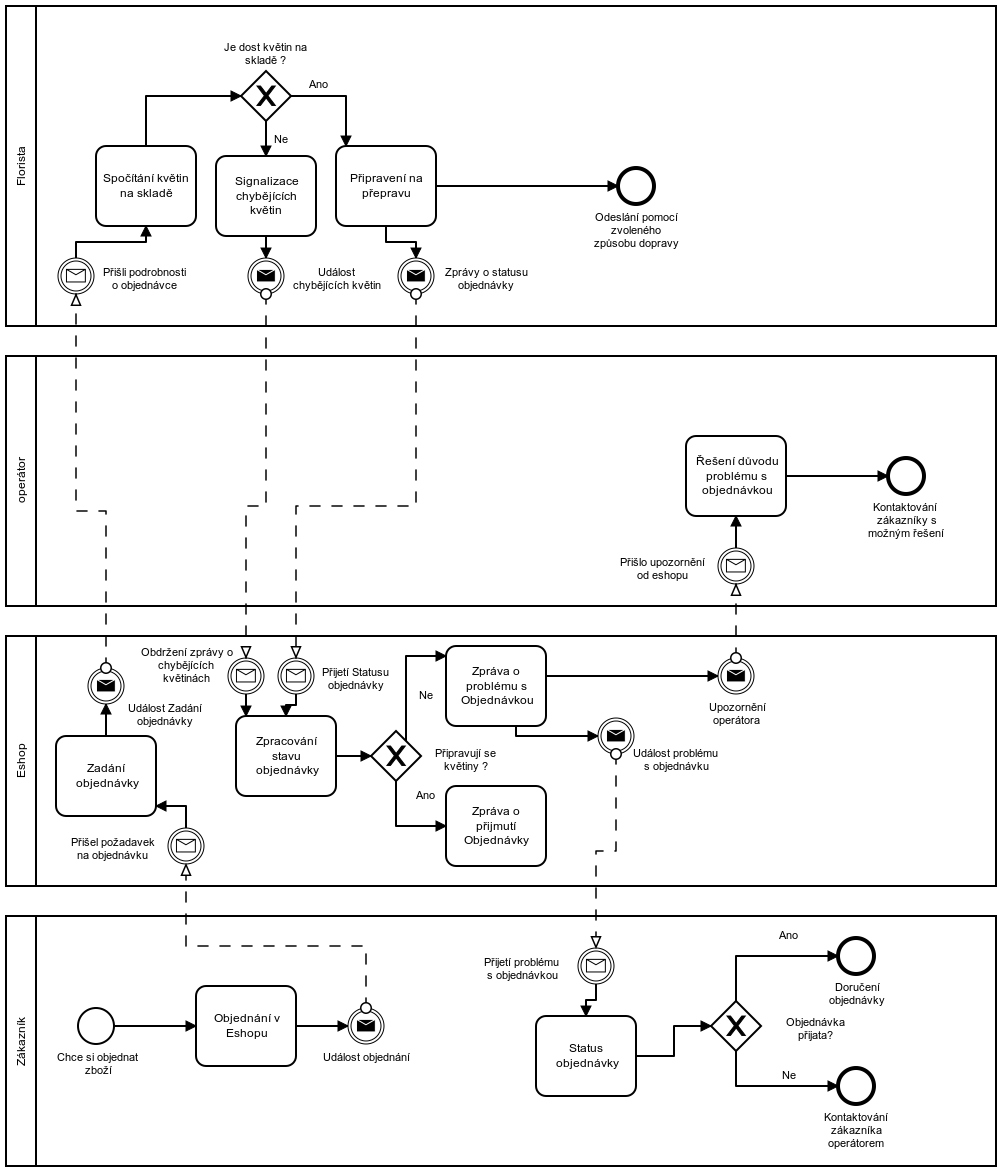
\includegraphics[width=\linewidth]{images/procesy/5.png}
\end{figure}

\newpage
\begin{figure}[h]
\caption{Vytvoření objednávky přes telefon}
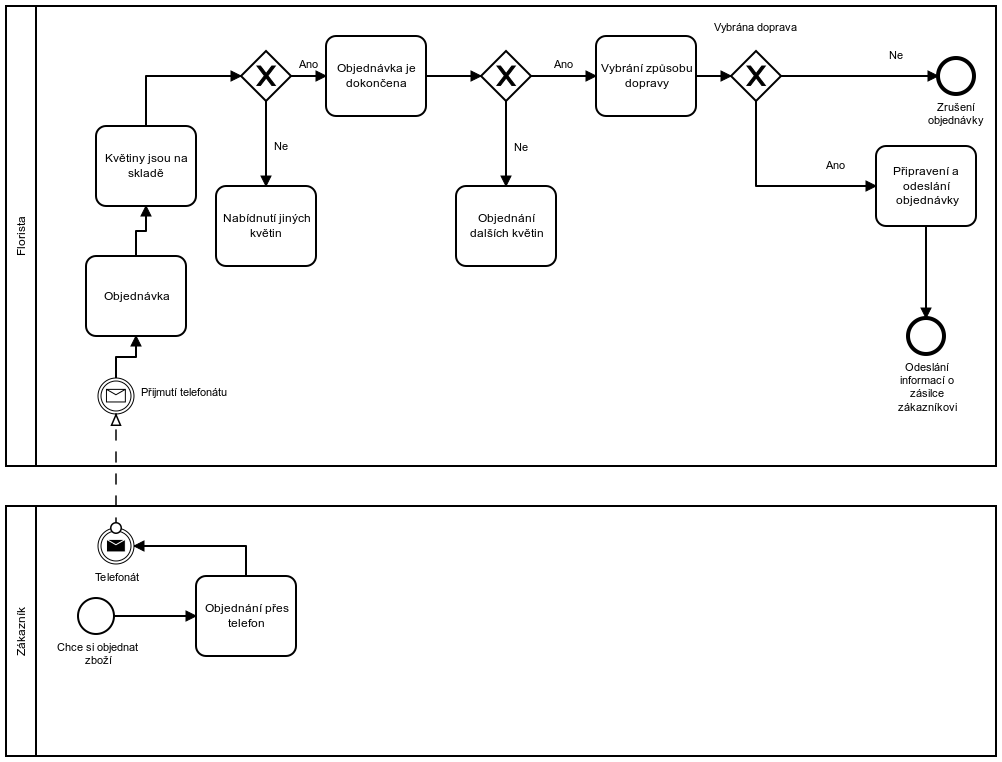
\includegraphics[width=\linewidth]{images/procesy/6.png}
\end{figure}

\newpage
\begin{figure}[h]
\caption{Vytvoření objednávky přes on-line službu (damekytky.cz)}
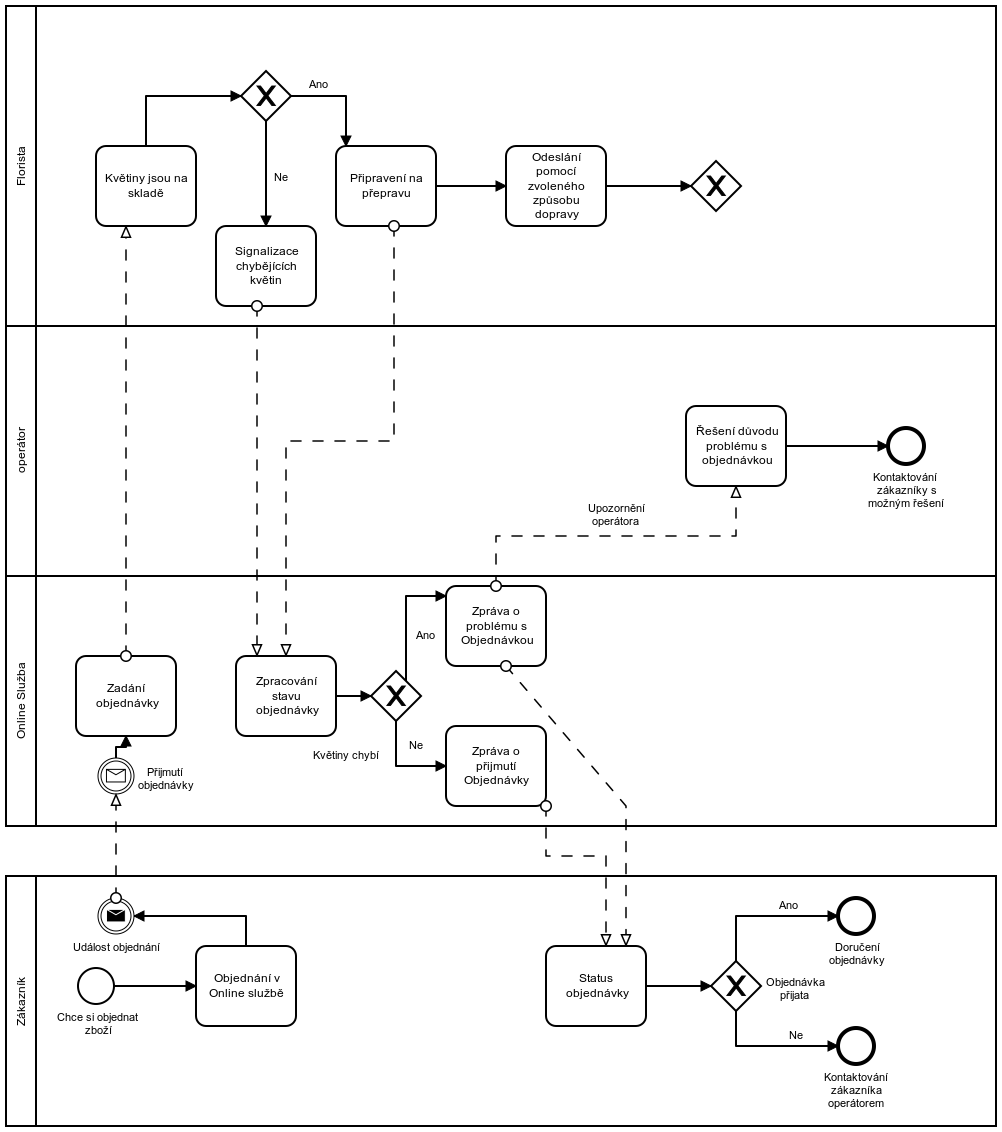
\includegraphics[width=\linewidth]{images/procesy/7.png}
\end{figure}

\newpage
\begin{figure}[h]
\caption{Příprava objednávky floristou}
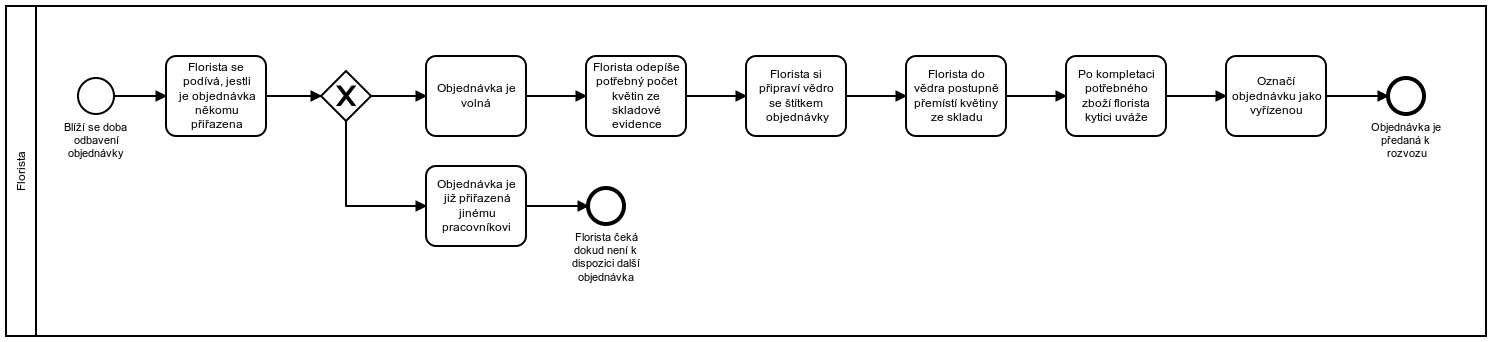
\includegraphics[width=\linewidth]{images/procesy/8.png}
\end{figure}

\newpage
\begin{figure}[h]
\caption{Distribuce připravené objednávky k zákazníkovi}
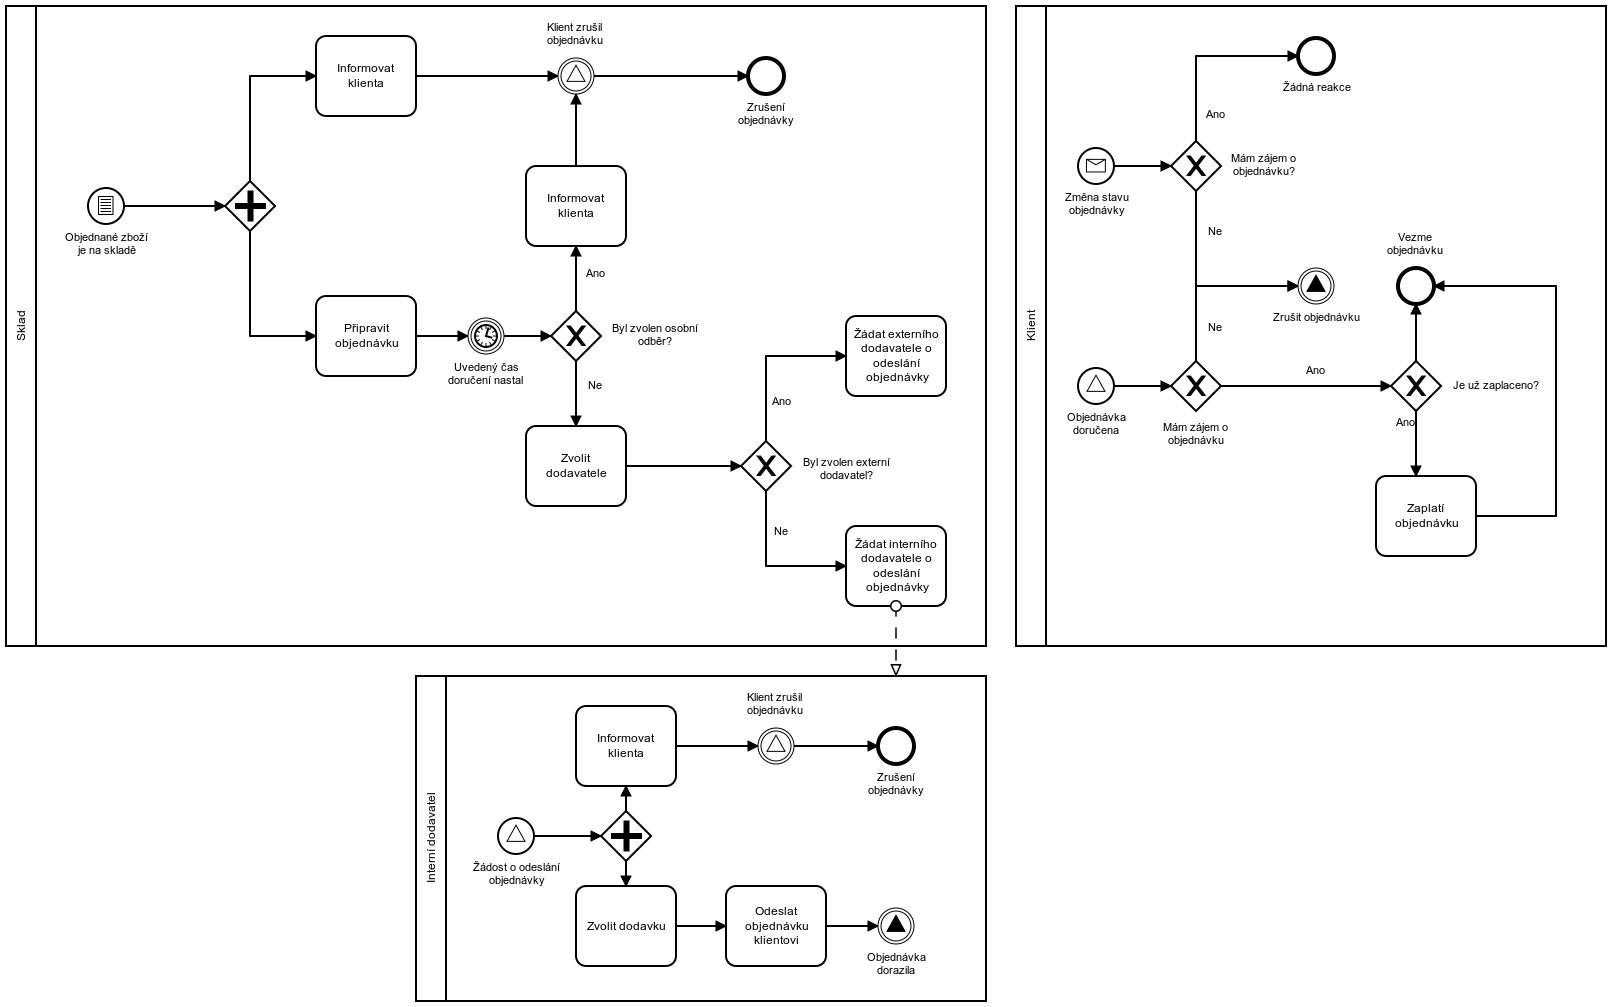
\includegraphics[width=\linewidth]{images/procesy/9.png}
\end{figure}

\newpage
\begin{figure}[h]
\caption{Reklamace při vyzvednutí osobně}
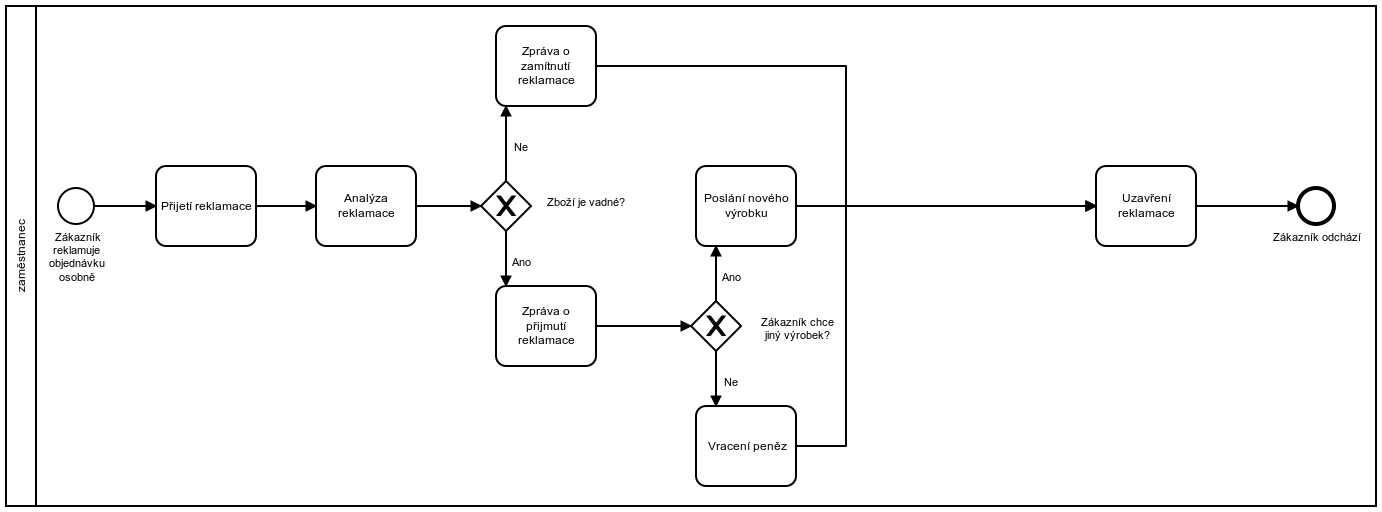
\includegraphics[width=\linewidth]{images/procesy/10.png}
\end{figure}

\newpage
\begin{figure}[h]
\caption{Reklamace objednávky při doručení kurýrem}
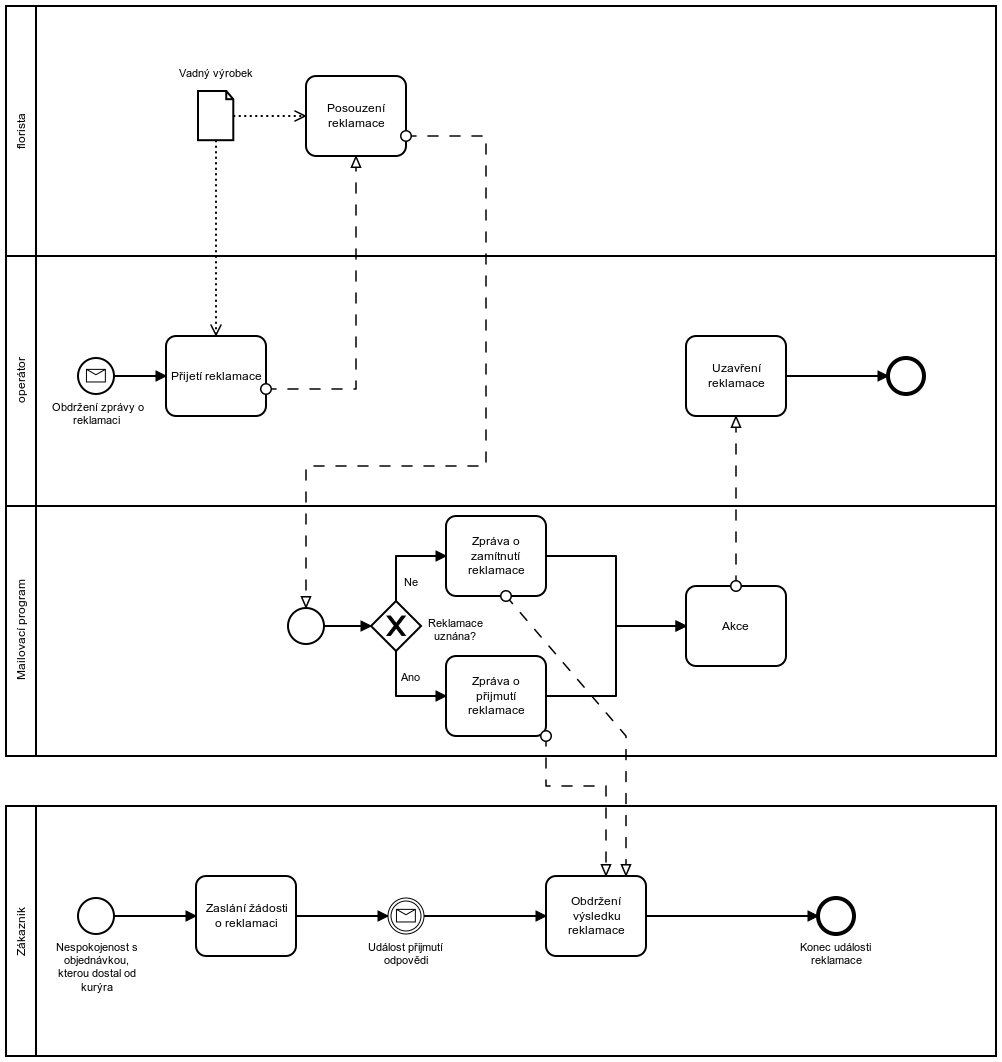
\includegraphics[width=\linewidth]{images/procesy/11.png}
\end{figure}

\newpage
\begin{figure}[h]
\caption{Sdílení reklamy}
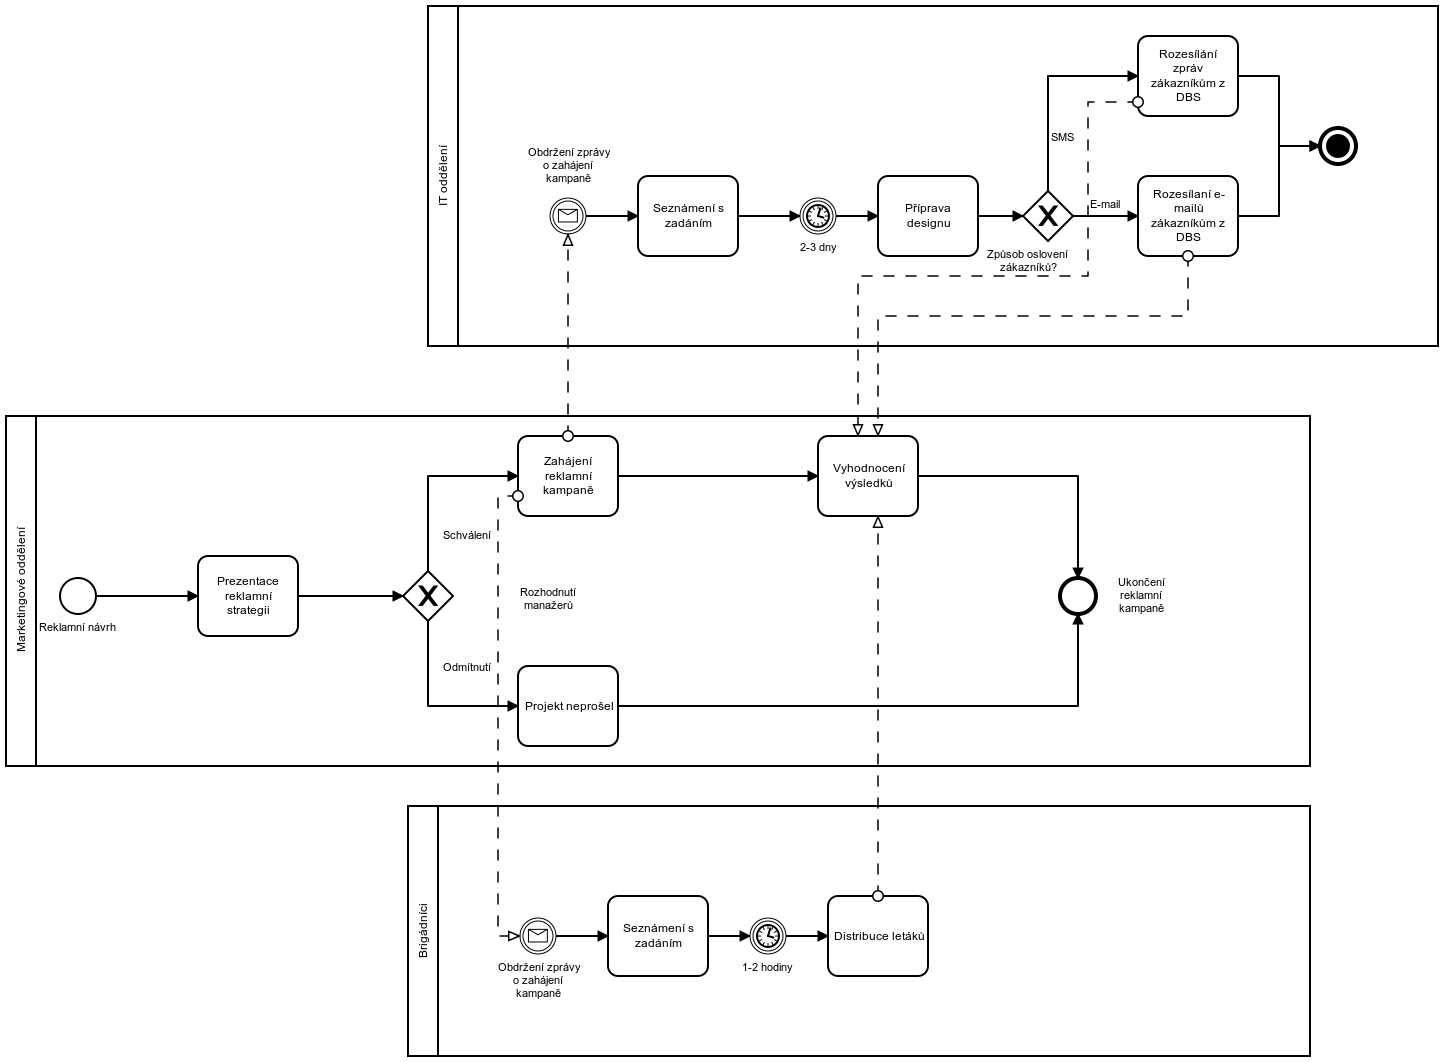
\includegraphics[width=\linewidth]{images/procesy/12.png}
\end{figure}

\newpage
\begin{figure}[h]
\caption{Kontrola zboží + přijetí zboží na pobočce}
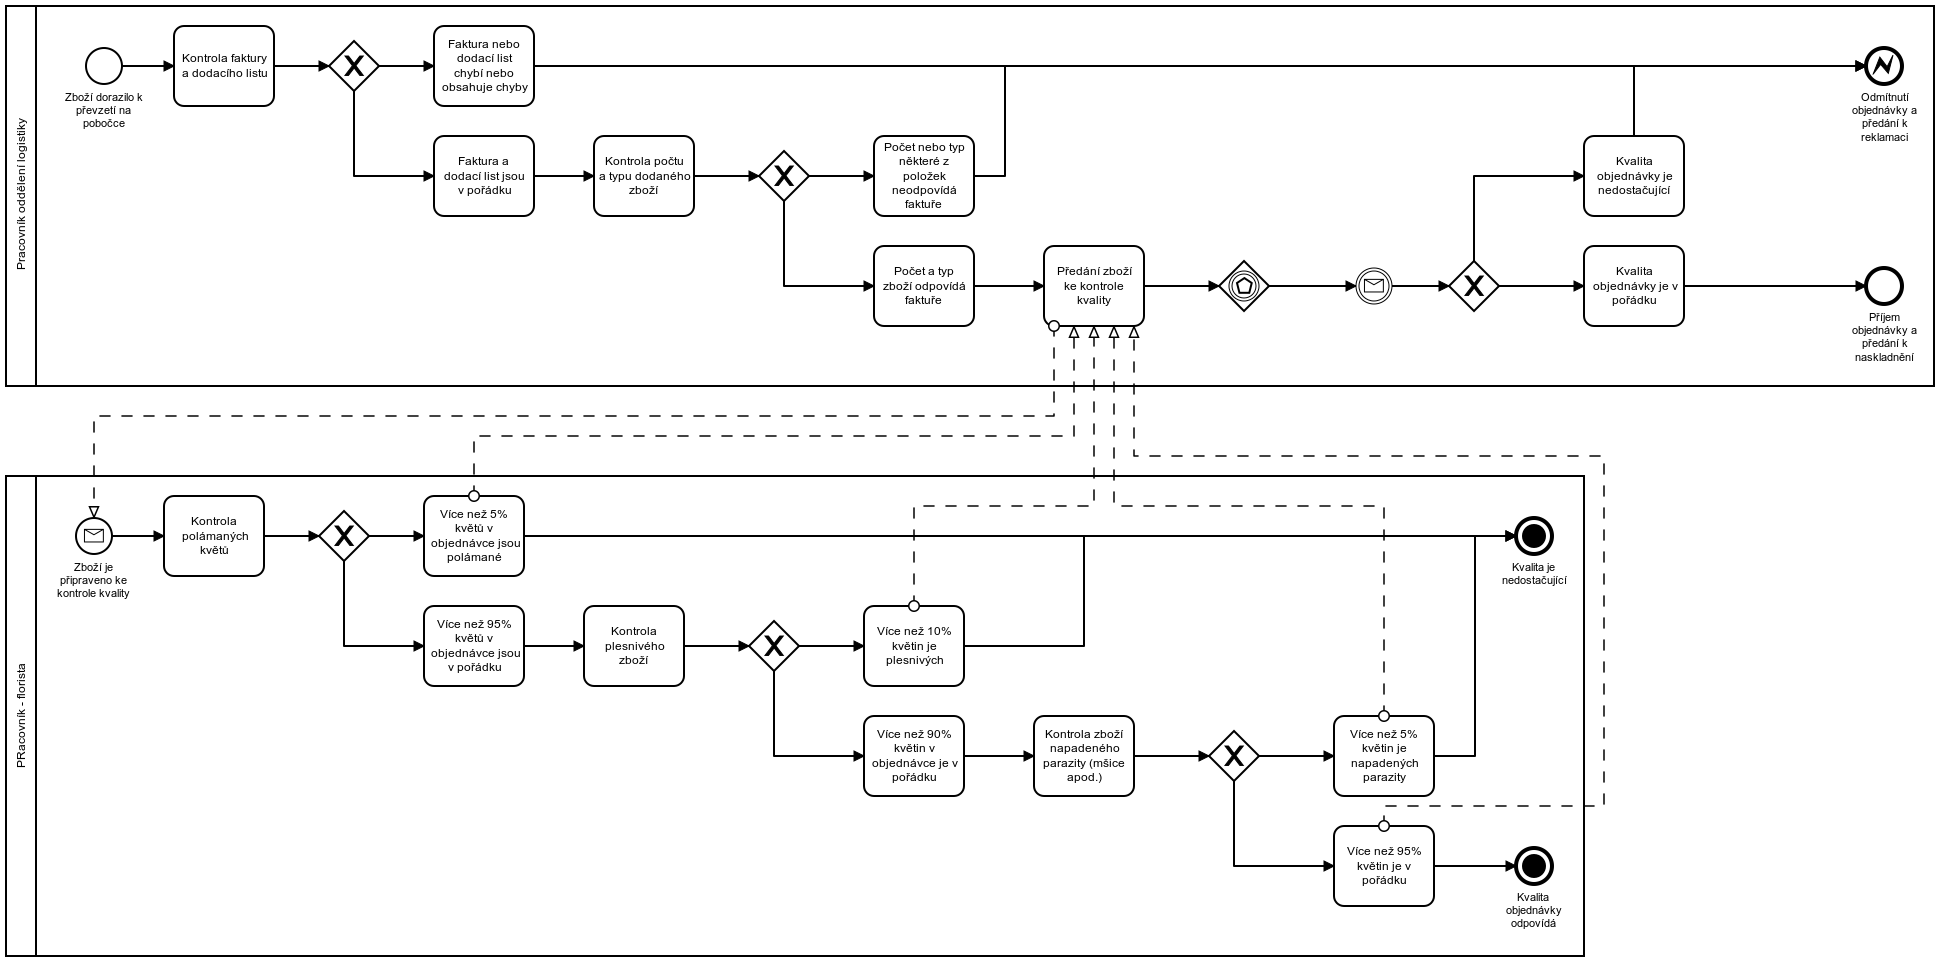
\includegraphics[width=\linewidth]{images/procesy/13.png}
\end{figure}


\newpage
\begin{figure}[h]
\caption{Plánování směn zaměstnanců}
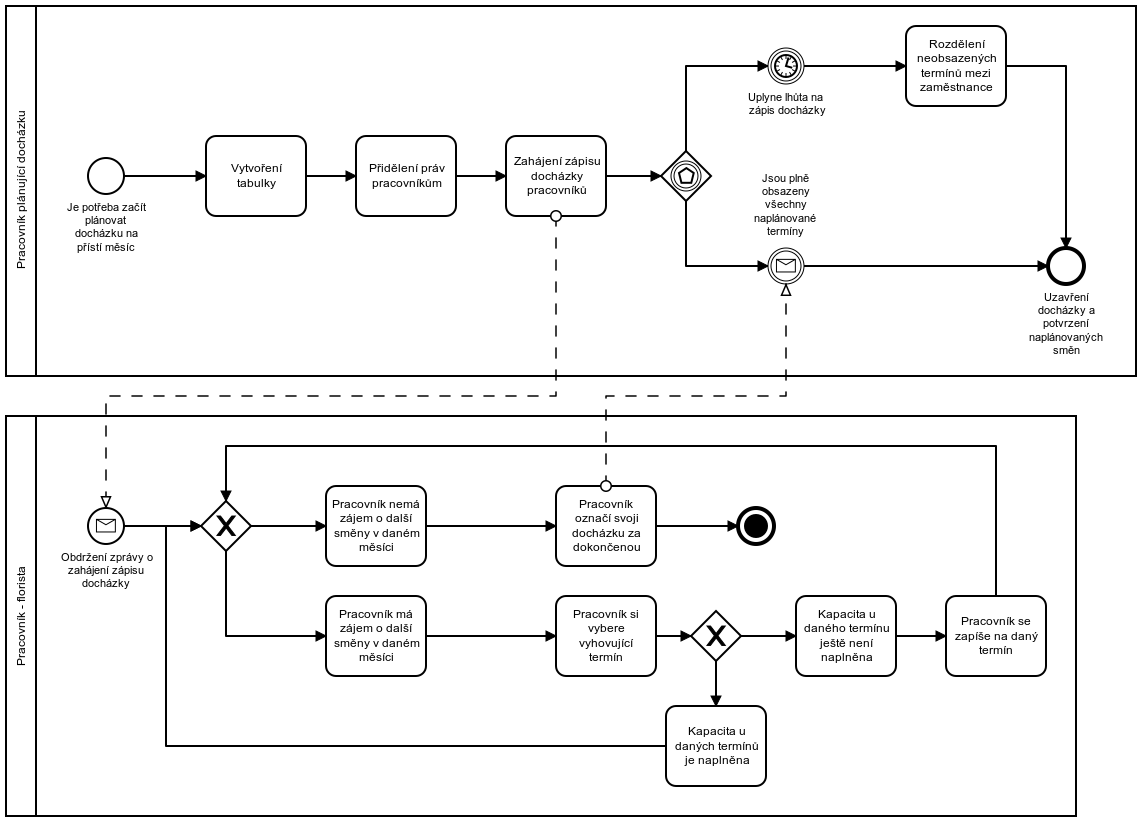
\includegraphics[width=\linewidth]{images/procesy/14.png}
\end{figure}

\newpage
\begin{figure}[h]
\caption{Uskladnění zboží + zadání do skladové evidence}
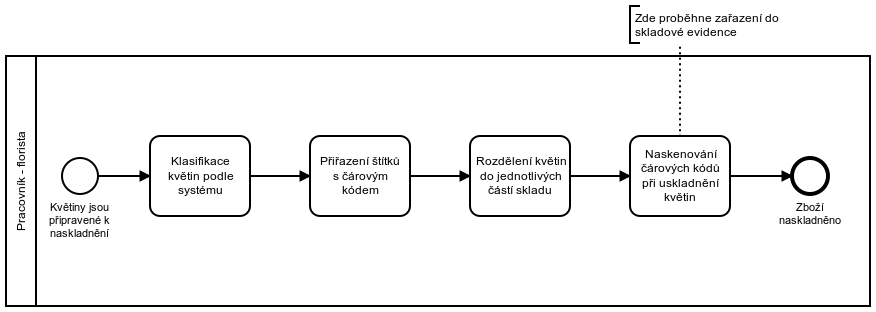
\includegraphics[width=\linewidth]{images/procesy/15.png}
\end{figure}

\newpage
\begin{figure}[h]
\caption{Vyřazení zkaženého zboží ze skladu}
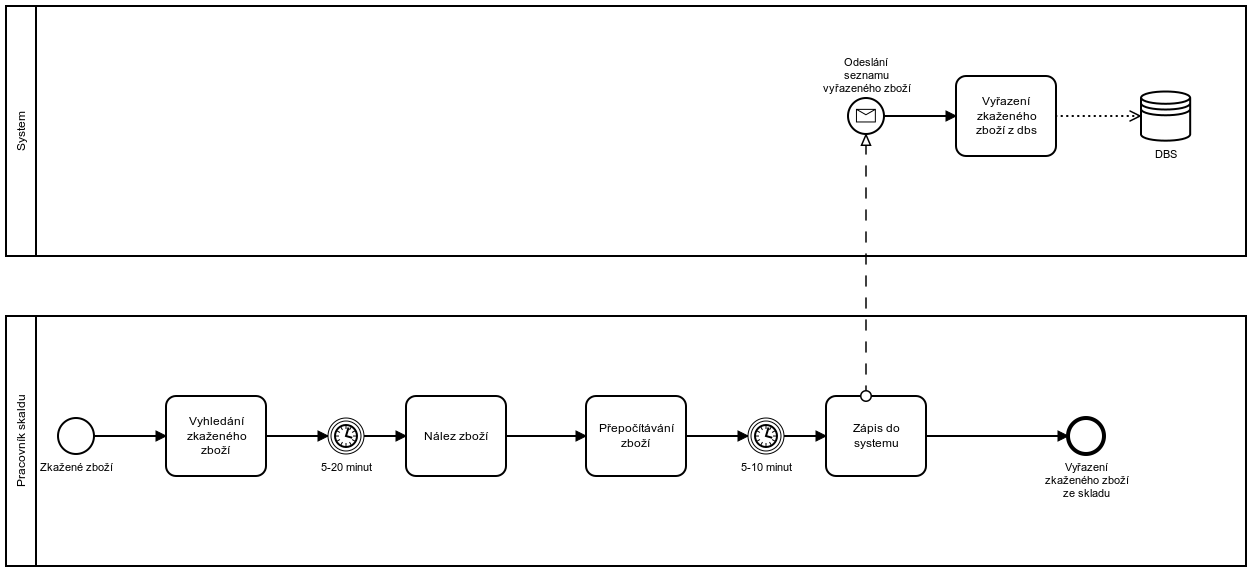
\includegraphics[width=\linewidth]{images/procesy/16.png}
\end{figure}

\newpage
\begin{figure}[h]
\caption{Ošetření květin před naskladněním}
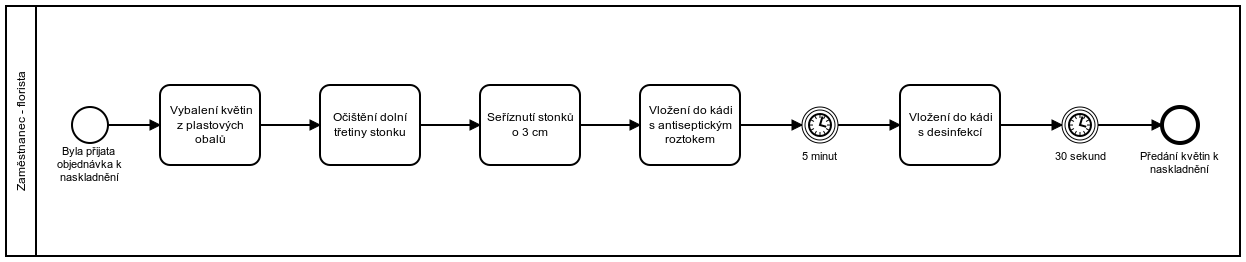
\includegraphics[width=\linewidth]{images/procesy/17.png}
\end{figure}

\newpage
\begin{figure}[h]
\caption{Zajištění komunikace se zákazníkem ohledně stavu objednávky}
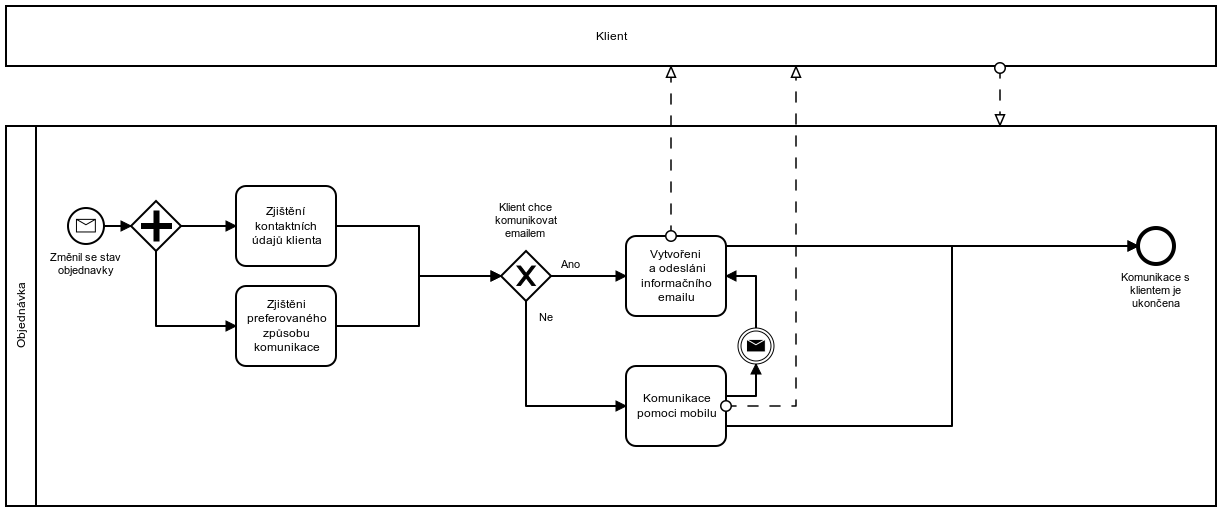
\includegraphics[width=\linewidth]{images/procesy/18.png}
\end{figure}

\newpage
\begin{figure}[h]
\centering
\caption{Real time komunikace s uživatelem e-shopu (chat)}
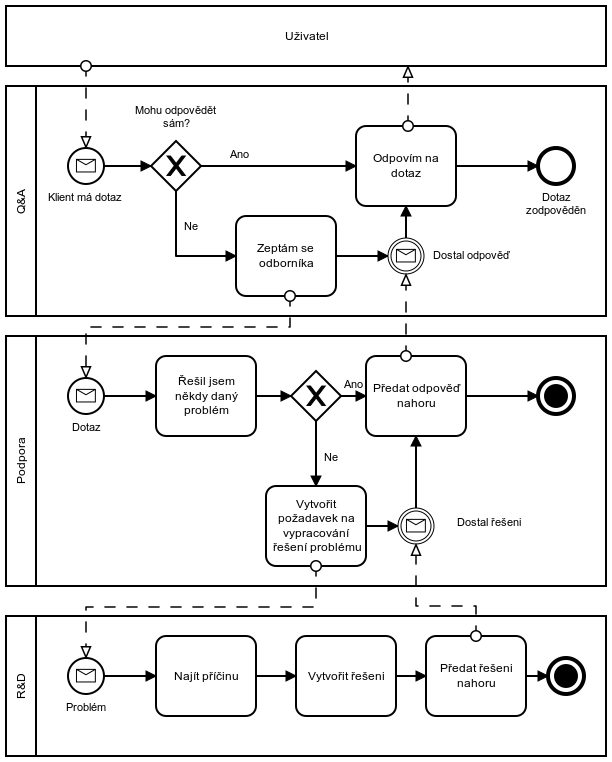
\includegraphics[width=\dimexpr\linewidth-50pt\relax]{images/procesy/19.png}
\end{figure}

\newpage
\begin{figure}[h]
\caption{Hiring nových zaměstnanců}
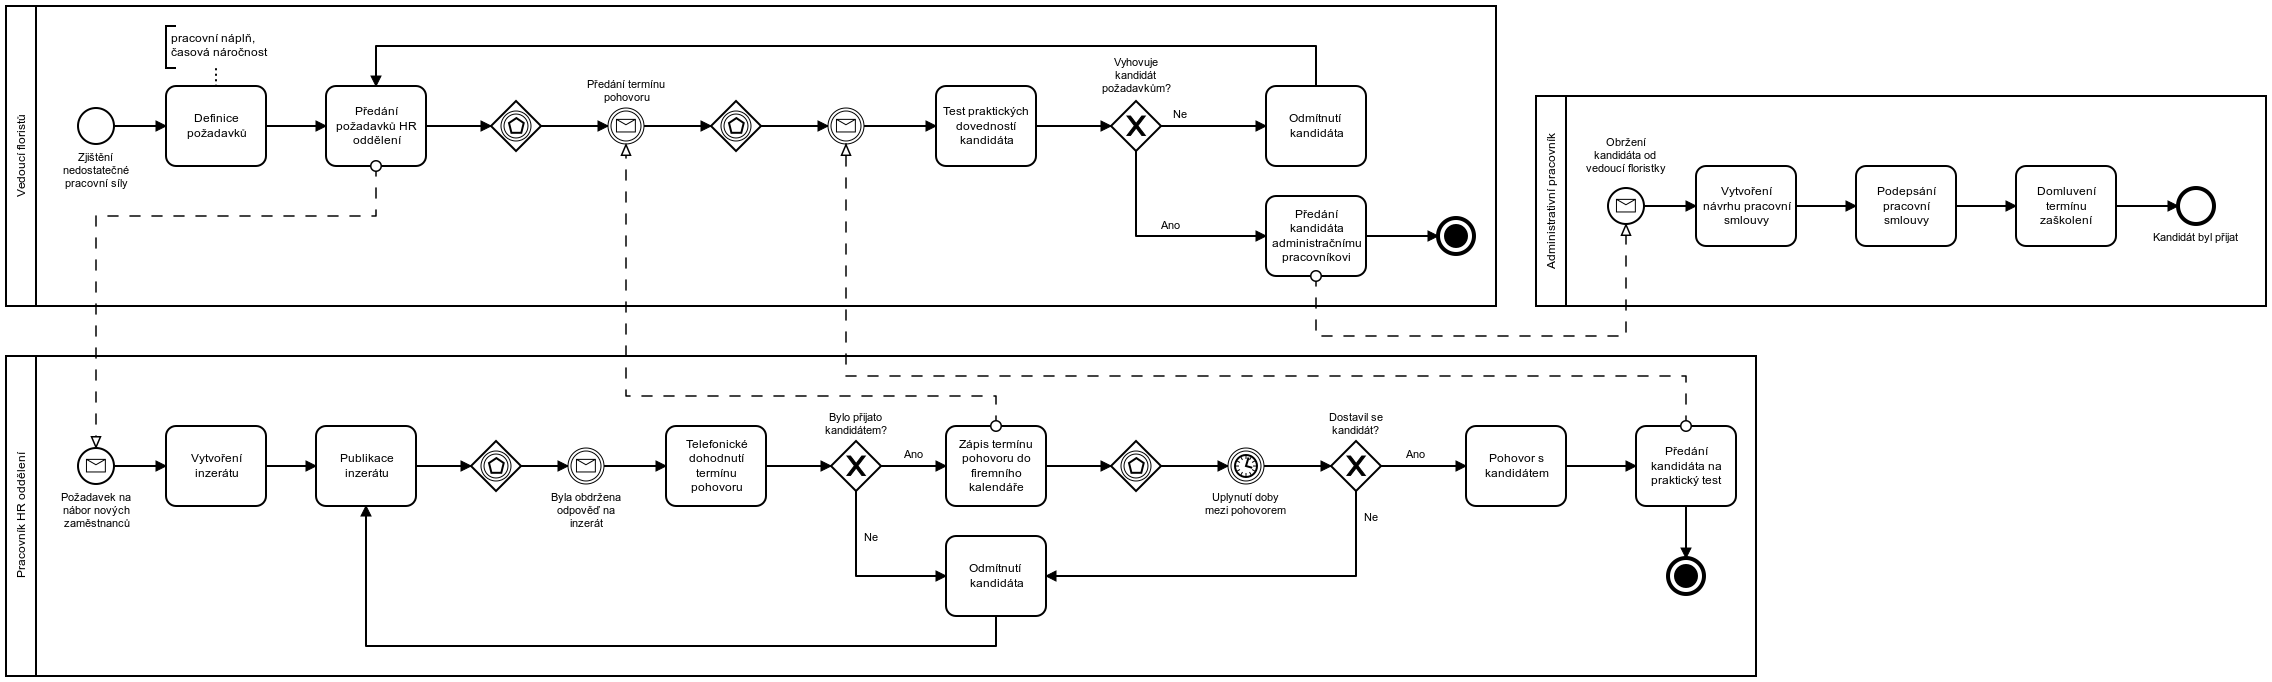
\includegraphics[width=\linewidth]{images/procesy/20.png}
\end{figure}

\newpage

\subsection*{Souhrnná analýza stavu IT}

\subsubsection*{Strategické řízení IT}

\begin{enumerate}
    \item \textbf{Podporuje IS/IT dosažení podnikových cílů?} \\
         Ano, firma provozuje e-shop, kde je možné si objednat květiny.
         Následně se objednávky zpracovávají za účelem vylepšení kvality poskytovaných služeb.

    \item \textbf{Je kvalita poskytovaných IT služeb dostatečná, nebo naopak nízká kvalita IT služeb ohrožuje kontinuitu a konkurenceschopnost byznysu?} \\
        Kvalita poskytovaných IT služeb není dostatečná, bez investice do informačního systému,
        který by propojil jednotlivé části společnosti není možné firmu dále škálovat a není možné
        zefektivnit produkci objednávek.


    \item \textbf{Existuje strategie podnikové informatiky?} \\
        Strategie podnikové informatiky existuje, ale není přesně a konkrétně definovaná.
        Celkovým cílem podnikové informatiky je zvýšení efektivity předávání informací mezi zaměstnanci.

    \item \textbf{Jsou definovány principy IT Governance (zodpovědnosti za klíčová rozhodnutí)} \\
        Nejsou definované přímo principy IT Governance, ale jsou definované zodpovědnosti za rozhodnutí jednotlivých pracovníků (např. při plánování docházky, dopravy nebo nákupu zboží na Holandské burze)


\end{enumerate}

\subsubsection*{Organizace vývoje a provozu IT}

\begin{enumerate}
    \item \textbf{Jsou nadefinovány a dodržovány IT procesy?} \\
        IT procesy nejsou ve firmě definovány, vývoj systémů (primárně nových Excel tabulek) je řízen on-demand.

    \item \textbf{Jsou IT procesy dobře měřeny?} \\
        IT procesy měřeny nejsou, jediná relevantní metrika, o které jsou bedeny záznamy je doba vývoje nových částí, od kterých se odvíjí výplaty IT pracovníků.

    \item \textbf{Vyhovuje organizace IT útvaru a rozdělení zodpovědností a pravomocí?} \\
        Organizace IT útvaru je naprosto nedostačující pro dané potřeby firmy.

    \item \textbf{Dodržují projekty plánovaný harmonogram?} \\
        Vývoj projektů není vázán harmonogramem, nemohou ho tudíž dodržovat.
\end{enumerate}

\subsubsection*{Ekonomika současného IT}

\begin{enumerate}
    \item \textbf{Sledují se náklady na IT služby, IT procesy a IT zdroje dle potřebných hledisek?} \\
        Náklady na IT služby jsou definovány pouze v rámci výplaty pracovníků IT oddělení.
        Sledování procesů a IT zdrojů ve firmě úplně chybí.

    \item \textbf{Jsou stanovovány a řízeny přínosy IS/IT?} \\
        Přínosy IS/IT systémů nejsou nijak měřeny, protože neexistuje jednotný systém a přínosy Excel tabulek jsou těžko měřitelné.

    \item \textbf{Dodržují se plánované rozpočty projektů?} \\
    Ano, pokud je na projekt stanoven rozpočet, musí ho zaměstnanci dodržet.

    \item \textbf{V čem jsou klíčové problémy ekonomické efektivnosti IS/IT?} \\
        Největším problémem ekonomické efektivnosti systémů je, že se jedná o velice obecné řešení,
        které není přizpůsobeno potřebám jednotlivých pracovníků a je tudíž nákladné dělat i minimální změny.
\end{enumerate}

\subsubsection*{Architektura IT služeb}
\begin{enumerate}
    \item \textbf{Je zdokumentovaná?} \\
        Dokumentace je minimální a i malá zdokumentovaná část je z velké části neaktuální.

    \item \textbf{Hodnocení kvality služeb (dostupnost, doba odezvy, škálovatelnost, cena...)} \\
        Online e-shop je hostován na platformě webnode.cz a služba je spolehlivá, nicméně velice omezená co se týče vzhledu a funkcionality, je náročné dělat změny a není možné integrovat web do Excel tabulek, tudíž zaměstnanci musí zadávat data manuálně což je velký problém z pohledu škálovatelnosti.
\end{enumerate}

\subsubsection*{Aplikační architektura}
\begin{enumerate}
    \item \textbf{Je zdokumentovaná?}\\
        Částečně, primární datová architekura vychází z Excel tabulek používaných pro skladovou evidenci.

    \item \textbf{Existují duplicity, nekonzistence?} \\
        Ano, každá tabulka obsahující propojená data může mít jiný systém číslování, databáze zákazníků obsahuje duplikovaná ID. Tím, že se nepoužívá např. DBMS neexistují v tabulkách integritní ani doménová omezení.

        Existujíc duplicity, bohužel současný systém neumožňuje založit nového zákazníka a při tom kontrolovat existenci.

    \item \textbf{Je kvalita dat (shoda s realitou) dostatečná?} \\
        Pro základní práci a analýzy je dostatečná, je možné zjistit informace, které pracovník potřebuje, ale není možné zároveň efektivně popsat část domény se kterou zaměstnanec pracuje bez toho, aby vznikaly duplicity.

    \item \textbf{Existují duplicitní funkce v různých aplikacích?} \\
        Firma pro svojí IT činnost používá pouze jedinou aplikaci a to MS Excel.

    \item \textbf{Jsou aplikace dobře integrovány?} \\
        Vzhledem k tomu, že firma pro svojí IT činnost používá pouze jediný software, není potřeba zajišťovat integraci. Integrace s verzemi je zabudovaná přímo do MS Excel.
\end{enumerate}

\subsubsection*{Technologická architektura}
\begin{enumerate}
    \item \textbf{Je zdokumentovaná?} \\
        Neexistuje dokument, který by obsahoval konkrétní technologickou architekturu podniku. Pokud si některý ze zaměstnanců není jistý jak se s konkrétní tabulkou pracuje, zeptá se pracovníka IT.

    \item \textbf{Je výhodná pro všechny aplikace?} \\
        Neexistuje jednotný model. Podnik má pouze technické zadání poskytnuté vývojářem spravující konkrétní tabulku.

    \item \textbf{Je škálovatelná?} \\
        Technologická architektura škálovatelná není, vývoj jednotlivých komponent probíhá nezávisle a je tudíž náročné a nákladné propojit novou část se zbytkem firemního IT.

    \item \textbf{Odpovídá počet a doba výpadků jednotlivých komponent požadované dostupnosti IT služeb?} \\
        Výpadky firemního systému jsou poměrně vzácné (MS Excel je vcelku stabilní program), ale často dochází k výpadkům na straně e-shopu, důvodem je využívání externí služby, která je následně upravená nedostatečně kvalifikovanými pracovníky což vede ke snížení stability celého řešení.
\end{enumerate}

\subsubsection*{Personální zajištění současného IT}
\begin{enumerate}
    \item \textbf{Odpovídá počet, kvalifikace a zkušenosti pracovníků vývoje a provozu IS/IT požadavkům na IT služby?} \\
        Počet pracovníků je dostačující, ale není dostačující jejich kvalifikace, firmě by se určitě vyplatilo investovat více peněz do školení IT zaměstnanců.

    \item \textbf{Je zajištěn kvalifikační rozvoj IT pracovníků?} \\
        Při nástupu jsou pracovníci IT oddělení zaškolení jedním ze stávajících pracovníků, což stačí na to, aby vykonávali svoji práci, ale lepší školení a kvalifikační rozvoj by určitě celému oddělení prospělo.

    \item \textbf{Není příliš vysoká fluktuace IT pracovníků?} \\
        Pracovníci IT oddělení je jedna z nejvíce stabilních částí firmy z pohledu fluktuace zaměstanců. Největší fluktuace probíhá v oddělení floristů, kde je velké procento zaměstnanců tvořeno brigádníky a externisty.

    \item \textbf{Funguje tvorba nástupnictví?} \\
        IT ve firmě zajišťuje tým mladých a zdravých lidí, kteří nemají v plánu z firmy odejít.
\end{enumerate}

\subsubsection*{Externí dodavatelé produktů a IT služeb}
\begin{enumerate}
    \item \textbf{Je kvalita produktů a služeb IT dodavatelů shodná s našimi požadavky} \\
        Ano, kvalita jediného externího produktu (MS Excel) odpovídá požadavkům.

    \item \textbf{Jaká je spolehlivost a stabilita dodatavatelů?} \\
        Dodavatel software (Microsoft) je jednou z největších firem světa a tedy i velice stabilní dodavatel.
\end{enumerate}

\subsubsection*{Bezpečnostní aspekty současného IT}
\begin{enumerate}
    \item \textbf{Jak jsou časté výpadky aplikací a komponent technologické infrastruktury? Ohrožují výpadky kontinuitu byznysu?} \\
        Výpadky technologické infrastruktury nejsou časté, ale mohou nastat. Lidské chyby a lidská nespolehlivost -- faktory, které mohou způsobit výpadek nebo jiné technologické problémy. Výpadky samozřejmě mohou mít negativní vliv na kontinuitu podniku, ale nezpůsobí úplné zastavení. Jelikož zákazníci preferují nakupovat květiny na kamenné prodejně.

    \item \textbf{Je dobře zajištěna identifikace uživatelů do našeho IS?} \\
        Společnost má chaotickou evidenci objednávek. Proto identifikace uživatelů může být poměrně problematická. Často se objevují duplicitní hodnoty, někteří zákazníci mohou být vedeni i 2 - 3 záznamy.

    \item \textbf{Vychází bezpečnostní polity pro IS/IT z podnikových bezpečnostních politik?} \\
        Bezpečnostní politiky jsou definované pouze pro fyzický přístup do budovy, např. do skladu. Politika přístupů do např. administrace e-shopu je velice zanedbaná.

    \item \textbf{Jak často je testovaná a ověřována bezpečnost?} \\
        Bezpečnost není prakticky vůbec monitorovaná, e-shop funguje na staré, nezabezpečené verzi frameworku.

    \item \textbf{Je systém dobře zajištěn proti neoprávněnému užití funkcí IS a zneužití dat?} \\
        Není, v minulosti se stalo, že data unikla, ale problém zabezpečení nebyl nalezen a vyřešen. Přístup do administrace e-shopu je pod sdíleným účtem s plnými administrátorskými právy. V této oblasti se nabízí velké pole působnosti pro případná zlepšení.
\end{enumerate}

\end{document}
